\chapter{Implementácia}
V predošlej kapitole sme popísali návrh aplikácie, ale nevenovali sme sa implementáčným detailom.
Implementácia klienta a servera je odlišná. Na klientovi riešime implementačné detaily vzhľadu
stránky, zatiaľ co na serveri štruktúru entít a ich ukladanie v databáze.

\subsection{Klient}
Klient je implementovaný ako jednostránková webová aplikácia. Celý klient je napísaný v knižnici
\textit{React} a jazyku \textit{Typescript}. Typescript je nadmnožinou jazyka JavaScript, ktorá do
tohto dynamického a netypovaného jazyka pridáva statické typy. Vďaka tomu je kód menej náchylný na
chyby a výhodou je tiež automatické navrhovanie kódu, ktoré editor poskytuje, pretože vie, čo je
akého typu. V implementácii sme zvolili rôzne farby pre rozhranie pre bežného používateľa a pre
administrátora. Komponenty zobrazované na klientovi využívajú knižnicu \textit{Material-UI}, ktorá
obsahuje jednoduché komponenty, ktoré sú naštýlované poďla Google dizajnov.

Pri načítaní stránky sa používateľovi zobrazí prihlasovacie okno, cez ktoré sa má do aplikácie
prihlásiť. Ak používateľ ešte účet nemá, vie sa prekliknúť na registráciu.
\begin{figure}[H]
\centering
\begin{subfigure}{.5\textwidth}
  \centering
  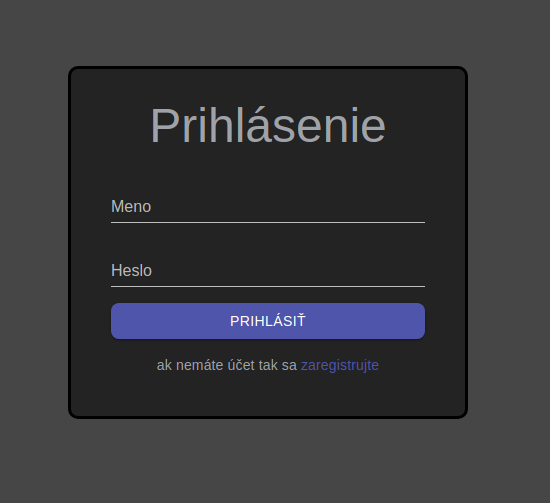
\includegraphics[width=0.8\textwidth]{images/prihlasenie}
  \caption[Prihlásenie]{Prihlásenie}
  \label{obr:prihlasenie}
\end{subfigure}%
\begin{subfigure}{.5\textwidth}
  \centering
  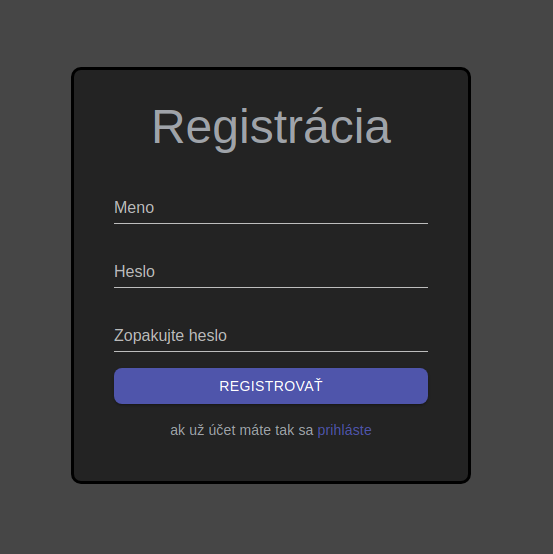
\includegraphics[width=0.8\textwidth]{images/registracia}
  \caption[Registrácia]{Registrácia}
  \label{obr:registracia}
\end{subfigure}
\caption{Prihlásenie a registrácia}
\end{figure}

Prihlasovací formulár validuje, či je používateľ zaregistrovaný a či zadal správne heslo. Podobne
registrovací formulár kontroluje, či je používateľské meno voľné a či sa heslá zhodujú. Prípadné
chyby zobrazuje pod formulárom.
\begin{figure}[H]
\centering
\begin{subfigure}{.5\textwidth}
  \centering
  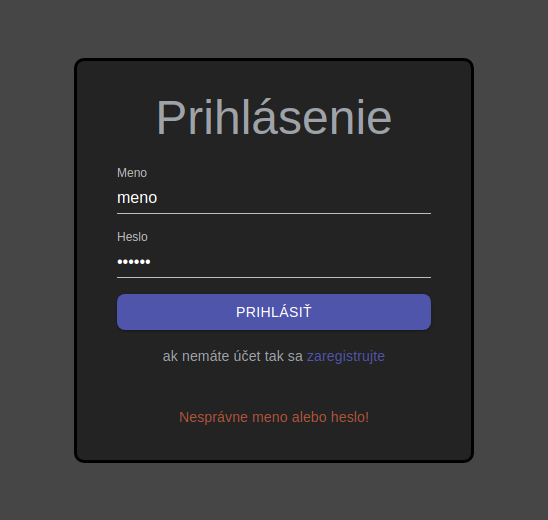
\includegraphics[width=0.8\textwidth]{images/validacia_prihlasenie}
  \caption[Validácia prihlásenia]{Validácia prihlásenia}
  \label{obr:validacia_prihlasenie}
\end{subfigure}%
\begin{subfigure}{.5\textwidth}
  \centering
  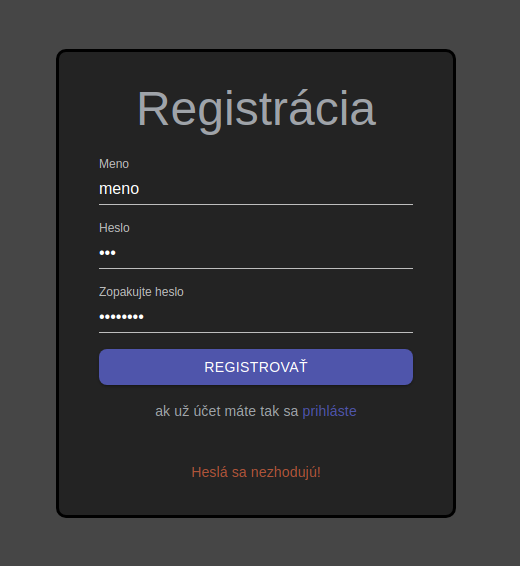
\includegraphics[width=0.8\textwidth]{images/validacia_registracia}
  \caption[Validácia registrácie]{Validácia registrácie}
  \label{obr:validacia_registracia}
\end{subfigure}
\caption{Validácia prihlásenia a registrácie}
\end{figure}

Po prihlásení používateľa sa zobrazí hlavná časť programu. Odlišuje sa však výrazne podľa toho, či
je prihlásený administrátor alebo bežný používateľ.

\subsection{Rozhranie pre bežného používateľa}
Pri implementácii rozhrania pre bežného používateľa sme použili kombináciu oďtieňov sivej na pozadia
a farby editoru a bielu farbu na písmo. Na výraznenie akcií, ktoré vie používateľ na stránke robiť,
používame špecifický odtieň modrej farby. Poslednou používanou farbou je červená, ktorou
singalizujeme chyby.

Po prihlásení sa zobrazí bežnému používateľovi rozhranie, v ktorom vidí všetky vytvorené skupiny.
Nevidí však ani ich obsah, ani prihlásených pouźívateľov patriacich do daných skupín. Do skupín
ho vie pridať iba administrátor. Ďalej sú v rozhraní zobrazené skupiny, do ktorých používateľ patrí
a v nich vidí aj ostatných pouźívateľov spolu so zadaniami pre danú skupinu.
\begin{figure}[H]
\centerline{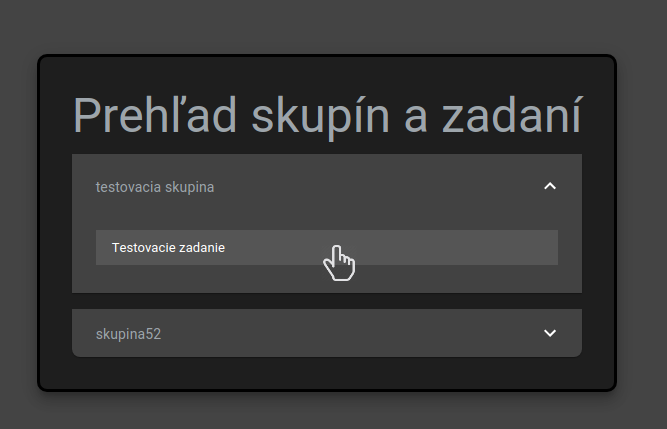
\includegraphics[width=0.7\textwidth]{images/vyber_zadania}}
\caption[Výber zadania]{Výber zadania}
\label{obr:vyber_zadania}
\end{figure}

Ak si používateľ vybral zadanie, otvorí sa mu editor, v ktorom vie upravovať všetky súbory dostupné
pre dané zadanie. Súčasťou editora sú viaceré komponenty, ktoré používateľovi uľahčujú a
zprehľadňujú prácu s editorom. 
\begin{figure}[H]
\centerline{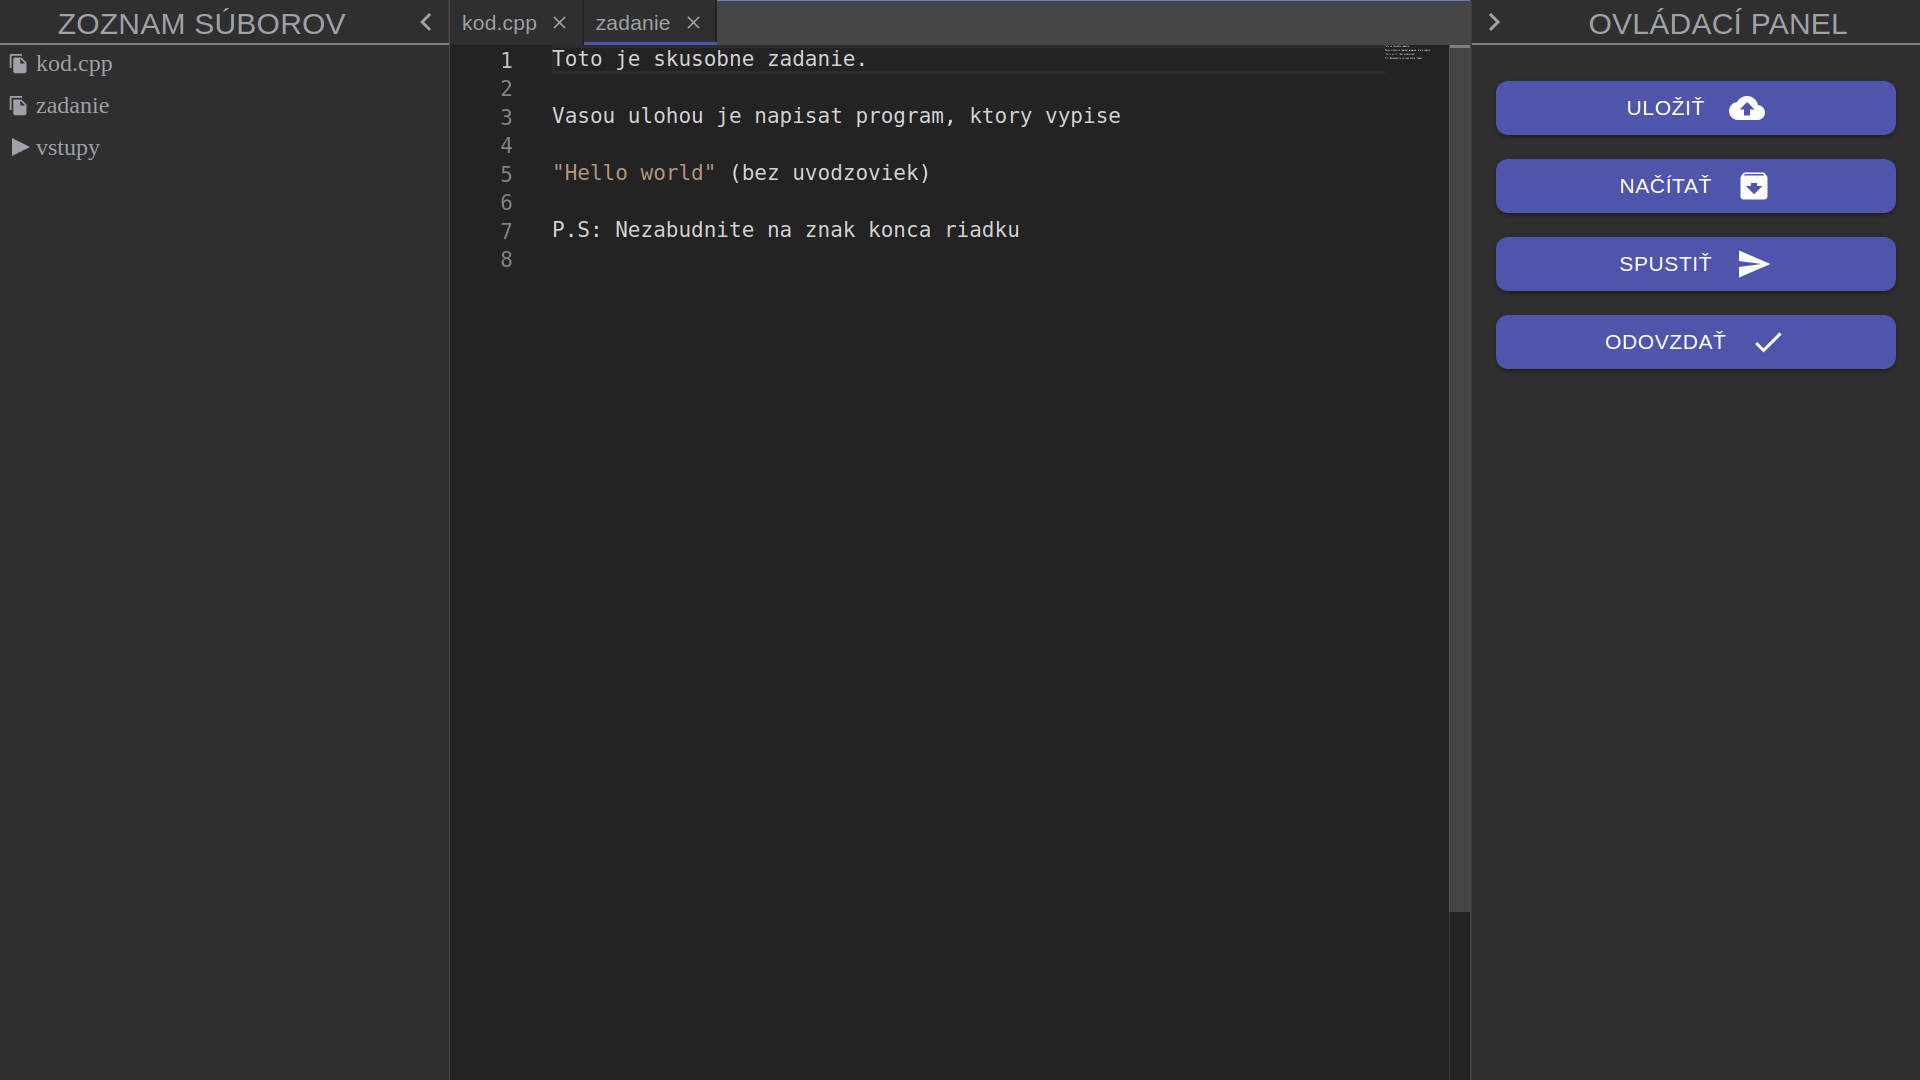
\includegraphics[width=1\textwidth]{images/bezny_pouzivatel}}
\caption[Editor zadania]{Editor zadania}
\label{obr:bezny_pouzivatel}
\end{figure}

% https://tex.stackexchange.com/questions/5035/paragraph-style-how-to-force-line-break-paragraph-make-paragraph-a-he
\paragraph{Panel so zoznamom súborov}\leavevmode\\
Komponent, ktorý obsahuje hierarchickú schému priečinkov a súborov dostupných v zadaní. Priečinky sa
dajú otvárať podobne ako pri otváraní súboru na počítači. Súbor alebo priečinok, na ktorý ukazuje
kurzor sa zvýrazňuje a kurzor sa zmení na ukazateľ, aby používateľ vedel, že môže na daný súbor
alebo priečinok kliknúť. Ikonky jasne odlišujú súbor od priečinku. Priečinok môže byť v schovanom
alebo zobrazenom stave. Tieto stavy sú rozlíšené typom ikonky.
\begin{figure}[H]
\centering
\begin{subfigure}{.5\textwidth}
  \centering
  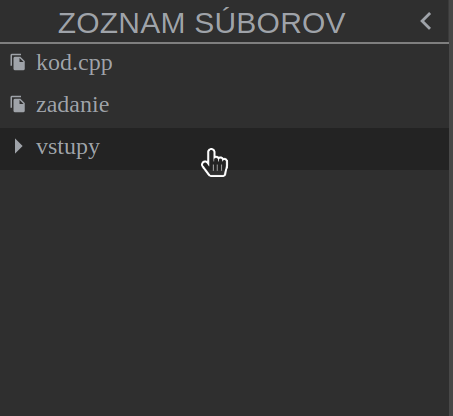
\includegraphics[width=0.8\textwidth]{images/schovany_zoznam}
  \caption[Schovaný obsah priečinka]{Schovaný obsah priečinka}
  \label{obr:schovany_zoznam}
\end{subfigure}%
\begin{subfigure}{.5\textwidth}
  \centering
  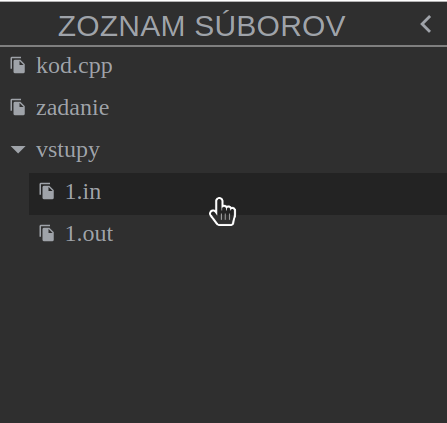
\includegraphics[width=0.8\textwidth]{images/zobrazeny_zoznam}
  \caption[Zobrazný obsah priečinka]{Zobrazný obsah priečinka}
  \label{obr:zobrazeny_zoznam}
\end{subfigure}
\caption{Priečinok v zozname súborov}
\end{figure}

% https://tex.stackexchange.com/questions/5035/paragraph-style-how-to-force-line-break-paragraph-make-paragraph-a-he
\paragraph{Ovládací panel}\leavevmode\\
Ovládací panel umožňuje používateľovi vykonávať akcie so svojím zadaním. Používateľ si môže svoj kód
uložiť, načítať, spustiť na vlastnom vstupe a otestovať na skrytých vstupoch tak ako to bolo 
napísané v návhu. Pri kliknutí na ľubovolnú akciu sa zobrazí dialóg, v ktorom používateľ doplní
ďalšie údaje a potvrdí akciu, ktorá sa následne vykoná na serveri.

Pri ukladaní zadania je nutné zvoliť identifikátor, pod ktorým sa má zadanie uložiť. Identifikátor
môže obsahovať ľubovolné znaky, no nesmie byť prázdny. Ak používaťel zadá neplatný 
identifikátor, klient mu súbor uložiť nedovolí.
\begin{figure}[H]
\centering
\begin{subfigure}{.5\textwidth}
  \centering
  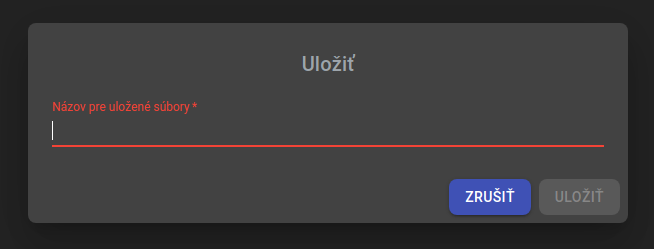
\includegraphics[width=0.8\textwidth]{images/neplatny_nazov}
  \caption[Neplatný názov identifikátora]{Neplatný názov identifikátora}
  \label{obr:neplatny_nazov}
\end{subfigure}%
\begin{subfigure}{.5\textwidth}
  \centering
  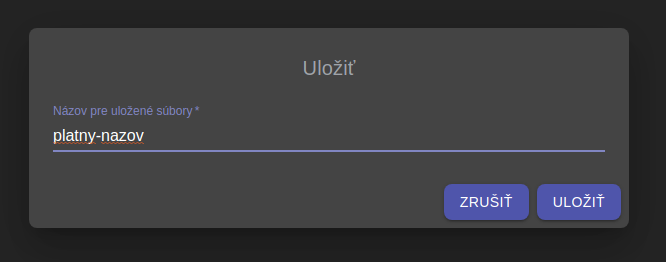
\includegraphics[width=0.8\textwidth]{images/platny_nazov}
  \caption[Platný názov identifikátora]{Platný názov identifikátora}
  \label{obr:platny_nazov}
\end{subfigure}
\caption{Uloženie zadania}
\end{figure}

Pri načítavaní uloženého zadania sa používateľovi zobrazia všetky jemu dostupné uložené zadania v 
zozname. Používateľ si vie vybrať, ktorý záznam chce načítať poďla identifikátora, ktorý zadával
pri ukladaní a časovej pečiatky, kedy záznam uložil. Okrem iného, aplikácia niekedy robí ukladanie
sama od seba. Používateľ si vie povedať, či chce takéto záznamy vidieť v možnostiach.
\begin{figure}[H]
\centering
\begin{subfigure}{.5\textwidth}
  \centering
  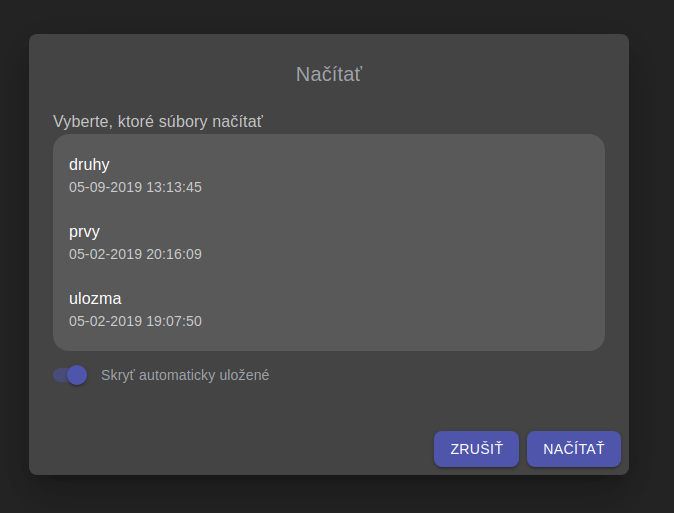
\includegraphics[width=0.8\textwidth]{images/nacitaj_zadanie}
  \caption[Iba vlastné uloženia]{Iba vlastné uloženia}
  \label{obr:nacitaj_zadanie}
\end{subfigure}%
\begin{subfigure}{.5\textwidth}
  \centering
  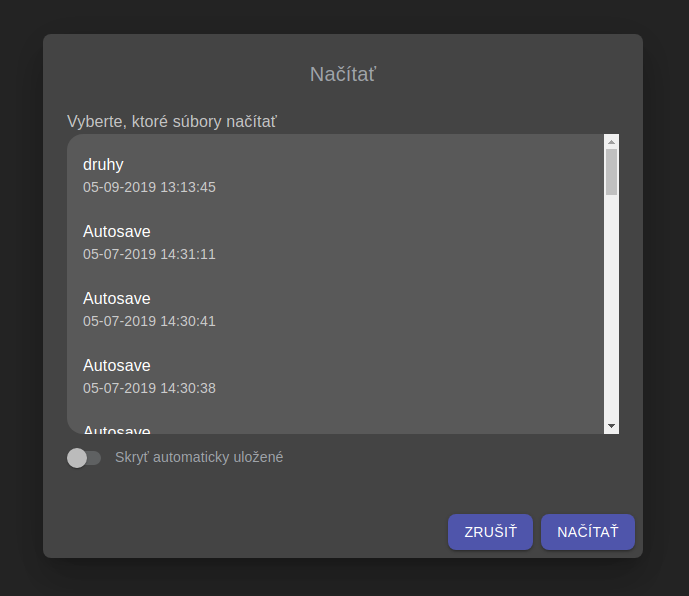
\includegraphics[width=0.8\textwidth]{images/nacitaj_automaticky_ulozene}
  \caption[Zobrazené aj automaticky uložené]{Zobrazené aj automaticky uložené}
  \label{obr:platny_nazov}
\end{subfigure}
\caption{Načítanie zadania}
\end{figure}

Po kliknutí na spustiť sa zobrazí dialóg, v ktorom vie používateľ zadať vlastný vstup a následne 
spustiť svoj program na danom vstupe. Užívateľ potom v dialógu potvrdí spustenie a program sa spolu
so vstupom ktorý zadal odošle na server, kde sa momentálny stav zadania automaticky uloží,
skompiluje a následne spustí. Počas behu programu sa v dialógu zmení tlačítko, ktoré upozorňuje, že
program beží. Po skončení behu programu sa zobrazí výsledný výstup v dialógu.
\begin{figure}[H]
\centering
\begin{subfigure}{.3\textwidth}
  \centering
  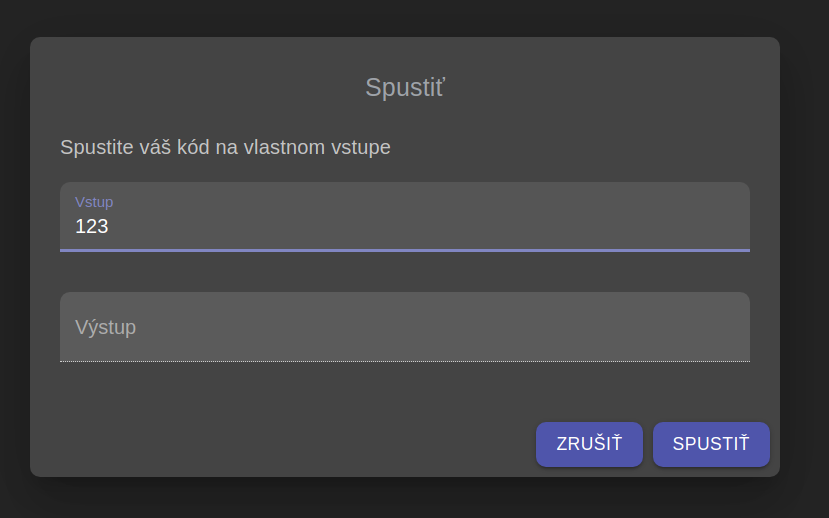
\includegraphics[width=0.9\textwidth]{images/spusti_dialog}
  \caption[Pred spustením]{Pred spustením}
  \label{obr:spusti_dialog}
\end{subfigure}%
\begin{subfigure}{.3\textwidth}
  \centering
  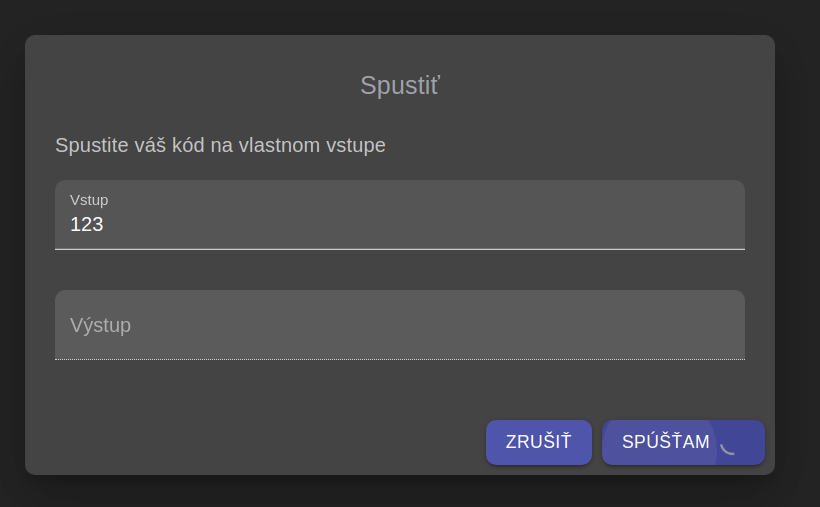
\includegraphics[width=0.9\textwidth]{images/spusti_dialog_beh}
  \caption[Počas behu]{Počas behu}
  \label{obr:spusti_dialog_beh}
\end{subfigure}
\begin{subfigure}{.3\textwidth}
  \centering
  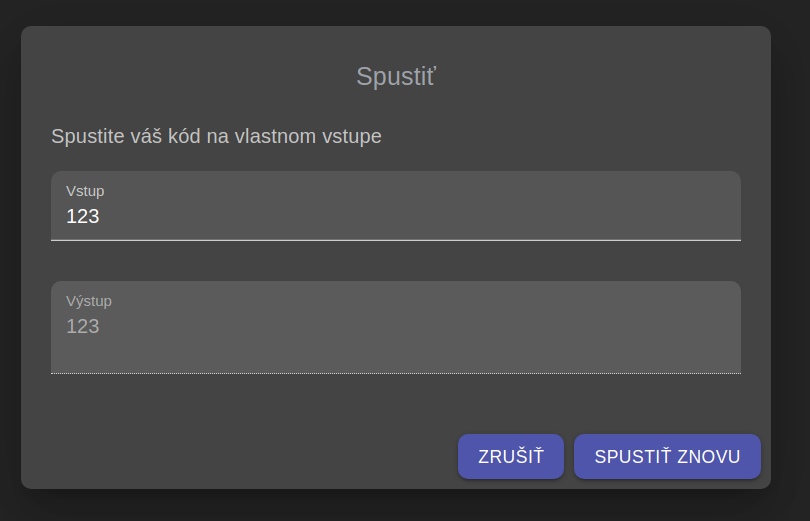
\includegraphics[width=0.9\textwidth]{images/spusti_dialog_koniec}
  \caption[Po dokončení]{Po dokončení}
  \label{obr:spusti_dialog_koniec}
\end{subfigure}
\caption{Spúštanie na vlastnom vstupe}
\end{figure}

Posledná akcia, ktorú vie používateľ spraviť je otestovanie svojho riešenia na skrytých vstupoch
uložených na serveri. Po kliknutí na tlačítko sa odošle na server aktuálny stav zadania, ktorý sa
na serveri uloží a automaticky začne testovať.
\begin{figure}[H]
\centering
\begin{subfigure}{.5\textwidth}
  \centering
  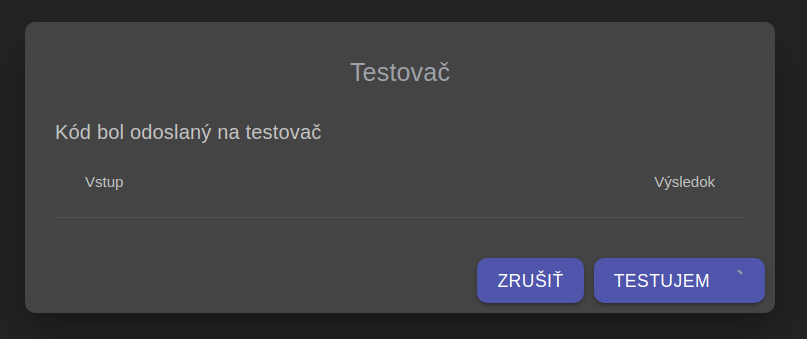
\includegraphics[width=0.8\textwidth]{images/testovanie_priebeh}
  \caption[Dialóg počas testovania]{Dialóg počas testovania}
  \label{obr:testovanie_priebeh}
\end{subfigure}%
\begin{subfigure}{.5\textwidth}
  \centering
  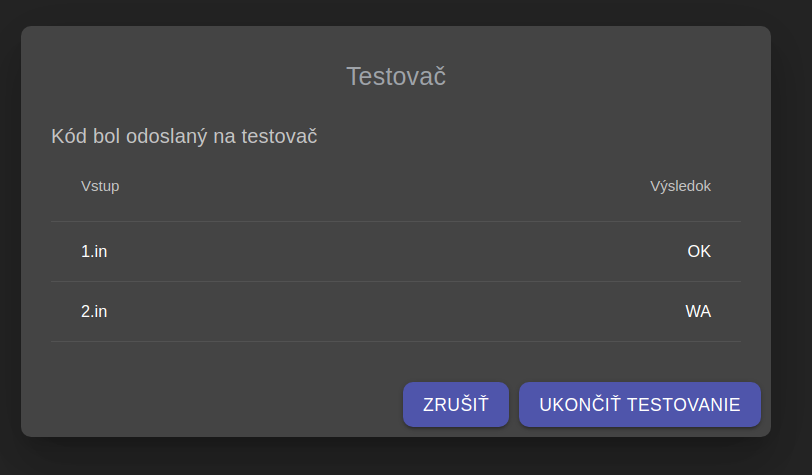
\includegraphics[width=0.8\textwidth]{images/testovanie_koniec}
  \caption[Dialóg po skončení testovania]{Dialóg po skončení testovania}
  \label{obr:testovanie_koniec}
\end{subfigure}
\caption{Testovanie na skrytých vstupoch}
\end{figure}

% https://tex.stackexchange.com/questions/5035/paragraph-style-how-to-force-line-break-paragraph-make-paragraph-a-he
\paragraph{Panel s otvorenými súbormi}\leavevmode\\
Dôležité je, aby používateľ vedel efektívne preklikávať medzi otvorenými súbormi a vedel, ktorý
súbor práve upravuje. Nato slúži horný panel editora, v ktorom sú zobrazené karty s práve otvorenými
súbormi. Aktívny súbor je podčiarknutý modrou farbou, aby bolo zvýraznené, ktorý súbor sa práve
upravuje. Súbory sa v hornom paneli dajú zavrieť v pravej časti karty klikom na krížik. Pri posune
kurzora nad oblasť krížika sa krížik zväčší, čím upozorní používateľa, že kliknutím zavrie danú
kartu. Používateľ môže medzi kartami prepínať, čím sa mení obsah editora.

% https://tex.stackexchange.com/questions/5035/paragraph-style-how-to-force-line-break-paragraph-make-paragraph-a-he
\paragraph{Editor kódu}\leavevmode\\
Najdôležitejším komponentom je samotný editor, v ktorom sa dá písať zdrojový kód. Editor použitý v
práci sa nazýva \textit{Monaco}, ktorý je použitý aj v populárnom editore \textit{VS Code}. 

Monaco automaticky zvýrazňuje syntax zdrojového kódu v práve otvorenom súbore. To, v ktorom jazyku
je zdrojový kód písaný, editor rozpozná podľa koncovky súboru. Monaco vie zobraziť syntax pre všetky
bežné programovacie jazyky, pričom sa dajú pridať ďalšie. V prípade, že sa editoru nepodarí
rozpoznať jazyk, v ktorom je obsah súboru napísaný, bude obsah zobrazený bez špeciálneho zvýraznenia
syntaxe.
\begin{figure}[H]
\centering
\begin{subfigure}{.5\textwidth}
  \centering
  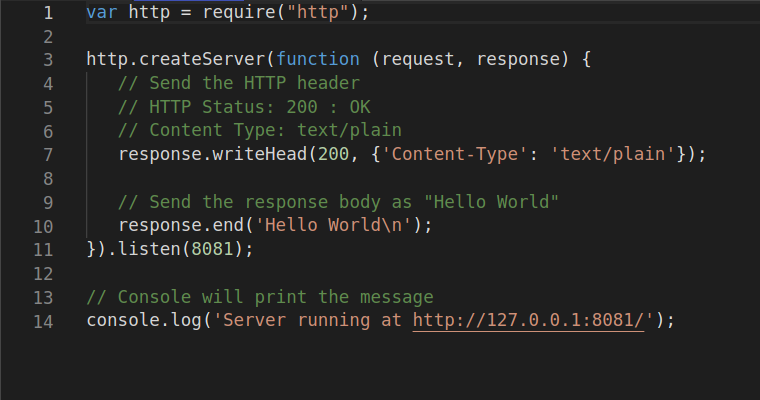
\includegraphics[width=0.8\textwidth]{images/jazyk_js}
  \label{obr:jazyk_js}
\end{subfigure}%
\begin{subfigure}{.5\textwidth}
  \centering
  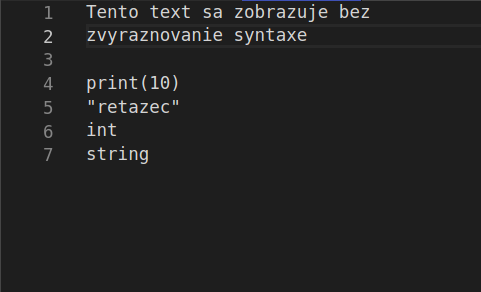
\includegraphics[width=0.7\textwidth]{images/jazyk_ziaden}
  \label{obr:jazyk_ziaden}
\end{subfigure}
\caption{Zvýrazňovanie syntaxe jazyka}
\end{figure}

Okrem zvýrazňovania syntaxe editor poskytuje základné operácie ako krok spať a krok dopredu. Pre
jednoduchšie navigáciu v texte je v pravej časti editoru "minimapka". Avšak najužitočnejšou a
najviac používanou funkcionalitou editora je nepochybne automatický návrh. Ak používateľ napíše pár
znakov, editor mu ponúkne na výber z možností, ktoré by mohol chcieť napísať. Používateľ môže
zobraziť návrh aj stlačením klávesovej skratky \textit{Ctrl + medzera}. Do návrhu sa postupne
pridávajú slová, ktoré používateľ do editoru napíše. V zozname navrhovaných možností sa používateľ
pohybuje šípkami a možnosť zvolí stlačením klávesy \textit{Enter}.
\begin{figure}[H]
\centerline{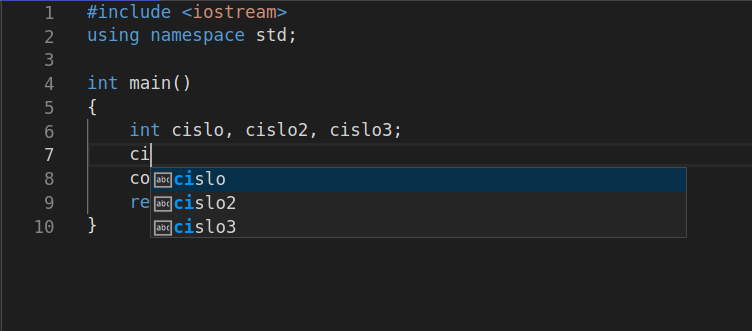
\includegraphics[width=0.7\textwidth]{images/automaticky_navrh}}
\caption[Automatický návrh]{Automatický návrh}
\label{obr:automaticky_navrh}
\end{figure}

Pri programovaní je dôležité vedieť v kóde nájsť nejaký reťazec, prípadne zmeniť nájdené výsledky na
nejaký iný reťazec. Monaco túto funkcionalitu podporuje po stlačení skratky \textit{Ctrl + F} pre
hľadanie a \textit{Ctrl + H} pre hľadanie spolu s nahradzovaním. Obe možnosti podporujú rôzne typy
vyhľadávania, ako napríklad hľadanie pomocou regulárnych výrazov. Na postupné označovanie nejakého
reťazca sa dá použiť aj multikurzor funkcionalita. Stačí, ak používateľ označí text a stlačí
\textit{Ctrl + D}. Tento príkaz nájde a označí ďalší výskyt s rovnakým textom aký používateľ
označil. 
\begin{figure}[H]
\centerline{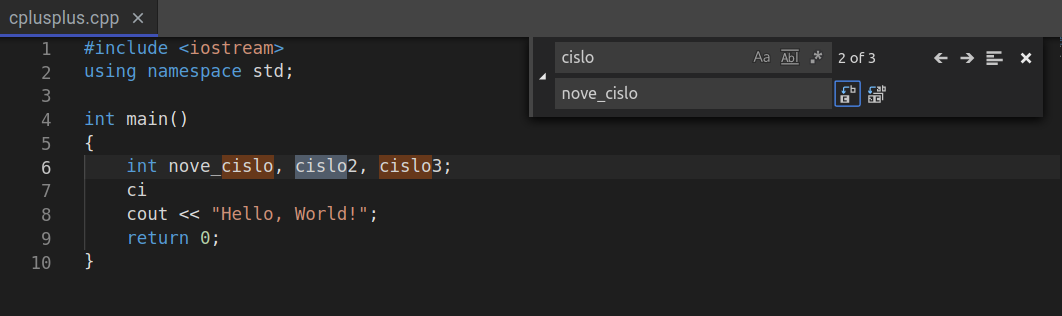
\includegraphics[width=0.7\textwidth]{images/hladanie_nahradzovanie}}
\caption[Hĺadanie a nahradzovanie]{Hĺadanie a nahradzovanie}
\label{obr:hladanie_nahradzovanie}
\end{figure}

Monaco obsahuje aj mnoho ďalších funkcii. Kompletný zoznam sa dá zobraziť stlačením klávesy
\textit{F1}. 

% https://tex.stackexchange.com/questions/5035/paragraph-style-how-to-force-line-break-paragraph-make-paragraph-a-he
\paragraph{Schované panely}\leavevmode\\
Oba panely zaberajú značný horizontálny priestor a nie vždy sú pre používateľa nutné. Má teda
možnosť panely schovať. Priestor, ktorý vznikne schovaním panelov vyplní editor. Používateľ môže
kedykoľvek panel zobraziť naspäť kliknutím na šípku, ktorá panel vyroluje a editor sa zmenší. 
\begin{figure}[H]
\centerline{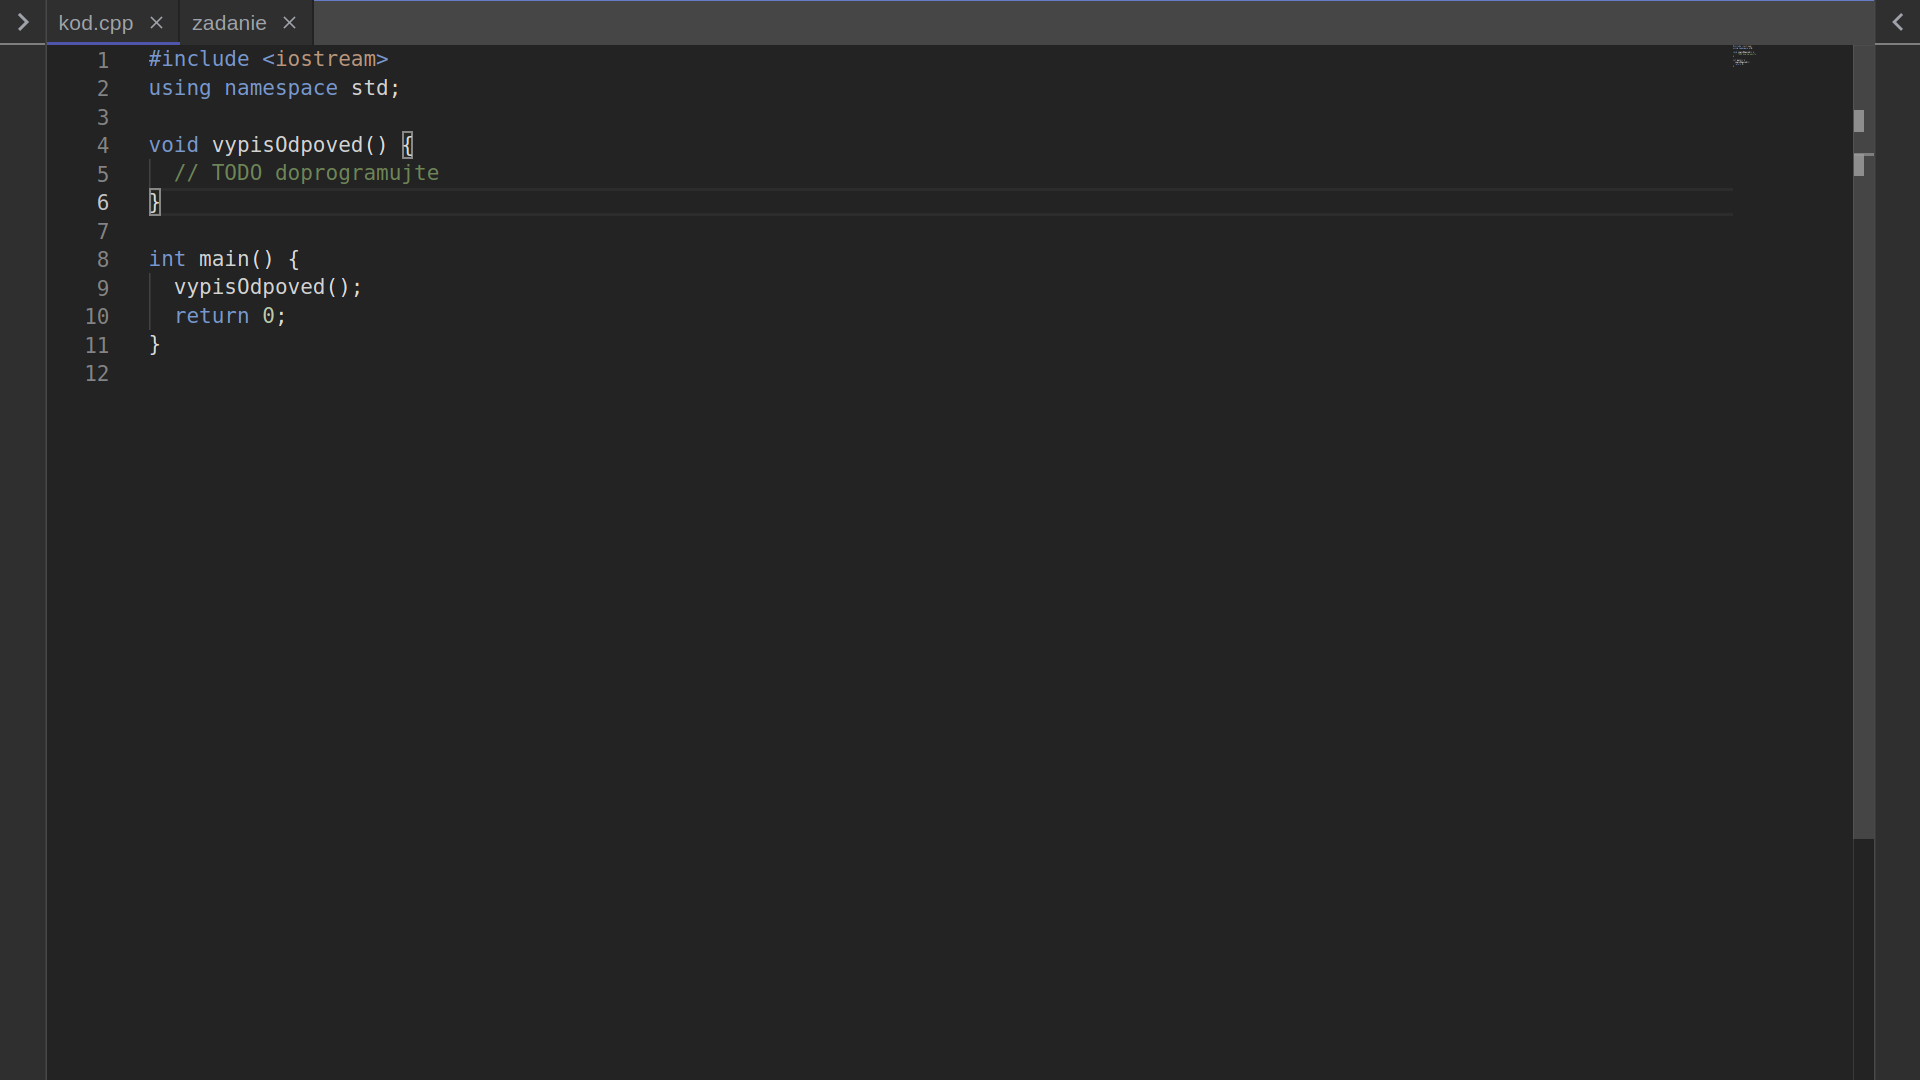
\includegraphics[width=1\textwidth]{images/zcucnute_panely}}
\caption[Editor zadania so schovanými panelmi]{Editor zadania so schovanými panelmi}
\label{obr:zcucnute_panely}
\end{figure}

\subsection{Rozhranie pre administrátora}
V návrhu aplikácie sme povolili registráciu iba pre bežného používateľa. Zároveň sme v aplikácii,
neumožnili žiaden spôsob ako spraviť z bežného používateľa administrátora. Vytvorenie administrátora
preto v klientskej aplikácii nie je možná. Administrátor sa dá vytvoriť iba pridaním
administrátorského účtu priamo do databázy na serveri. Keď sa adminsitrátor prihlási na klienta, 
zobrazí sa mu automaticky administrátorské rozhranie.

Farby použíté na rozhranie pre adminsitrátora sú úplne iné oproti farbám zvoleným na reozhranie pre
bežného používateĺa. Administrátorské rozhranie používa na pozadie bielu farbu a text používa farby
odtieňov sivej. Tieto farby sú predvolenými farbami knižnice \textit{React admin}, ktorá je použitá
na vytvorenie rozhrania. Jazyk použítý v rozhraní je anglický, pretože knižnica používa anglický
jazyk a preklad do slovenčiny by bol náročný a zdĺhavý.

React admin dovoľuje deklaratívne popísať administrátorské rozhranie a jediná požiadavka knižnice je
webová cestu, na ktorej je dostupný server. Aplikácia potom volá rozhranie servera a výsledné dáta
zobrazuje. Knižnica je veľmi užitočná, lebo sa dá použíť s ľubovolným typom servera, tiež používa
\textit{Material-UI} a využíva optimistické zobrazovanie. Veľkým bonusom je aj detailná dokumentácia
a aktívna komunita podporujúca túto knižnicu.

\begin{figure}[H]
\centerline{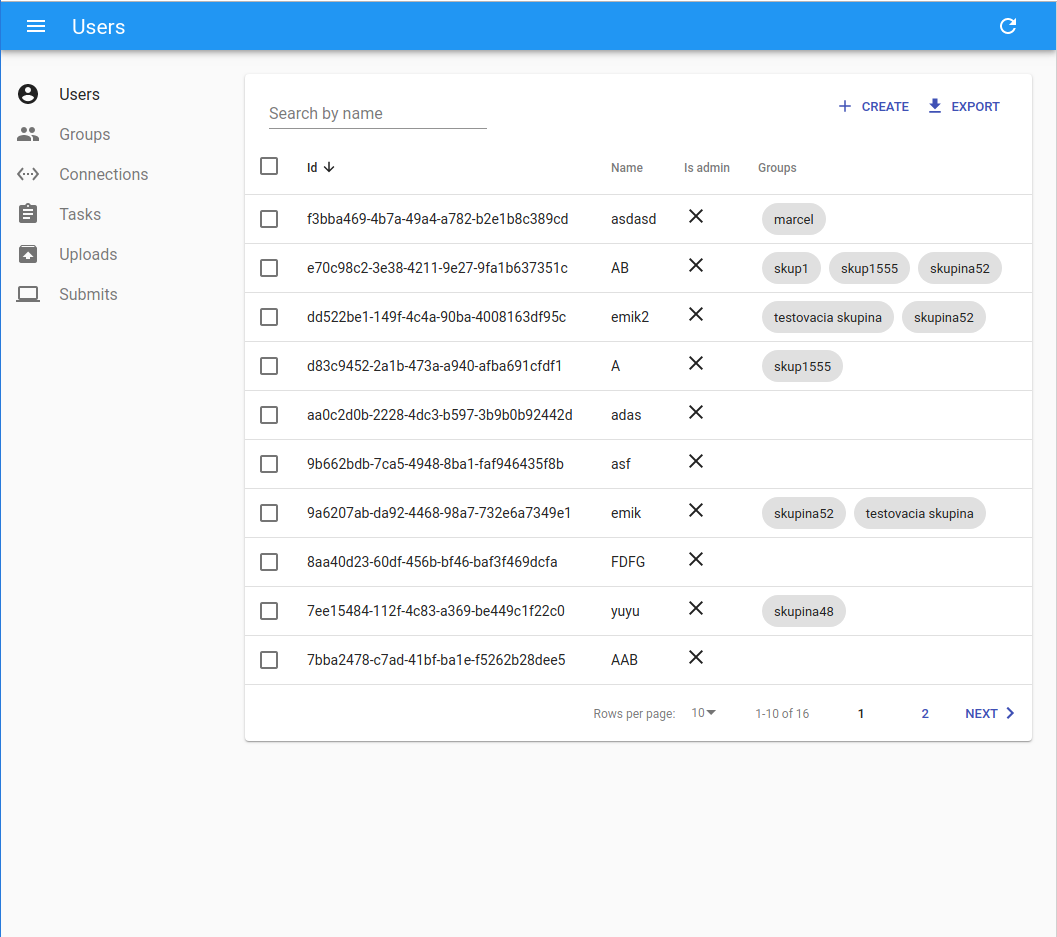
\includegraphics[width=1\textwidth]{images/administratorske_rozhranie}}
\caption[Administrátorské rozhranie]{Administrátorské rozhranie}
\label{obr:administratorske_rozhranie}
\end{figure}

Administrátorské rozhranie obsahuje navigačný panel, ktorý rozhoduje o tom, ktoré entity sú
zobrazované v hlavnej časti administrátorského rozhrania. Každý prvok v navigačnom paneli má vlasnú
ikonku a predstavuje rozdielnu časť rozhrania na serveri.

Hlavnú časť administrátorského rozhrania nazývame \textit{panel}. Panel má všeobecnú štruktúru,
ktorú rozdeľujeme na:
\begin{itemize}
  \item akcie
  \item tabuľka entít
  \item stránkovanie
\end{itemize}

% https://tex.stackexchange.com/questions/5035/paragraph-style-how-to-force-line-break-paragraph-make-paragraph-a-he
\paragraph{Akcie}\leavevmode\\
Akcie sa nachaazjú v hornej časti panela a štandardne je v knižnici React admin implemntovaná iba
akcia \textit{exportovať}, ktorá vytvorí CSV súbor so všetkými entitami zobrazenými v tabuľke.
Ďalšie akcie sa však dajú pridať a vačšina panelov má implementovanú aspoň akciu \textit{vytvor},
ktorá ponúkne jednoduchý formulár na vyplnenie údajov entity, ktorý sa následne odošle na server,
kde sa uloží do databázy. Okrem toho poskytuje knižnica možnosť vytvoriť si filtre. Filtre len
pridávajú parametre, ktoré sa posielajú spolu s požiadavkou na rozhranie servera. Samotné
filtrovanie sa vykonáva až na serveri. 

% https://tex.stackexchange.com/questions/5035/paragraph-style-how-to-force-line-break-paragraph-make-paragraph-a-he
\paragraph{Tabuľka entít}\leavevmode\\
Tabuľka entít zobrazuje dáta, ktoré vráti rozhranie servera. Názvy stĺpcov tabuľky śu klikateľné a
služia na triedenie zobrazovaných výsledkov. Podobne ako pri filtrovaní, knižnica iba posiela 
parametre na server, ktorý zodpovedá za to aby vrátené výsledky boli správne utriedené.
Po kliknutí na riadok tabuľky sa zobrazí detailný popis danej entity. Knižnica umožňuje aj meniť 
údaje entít, záleží na tom, či chceme aby sa daná entita, prípadne nejaká jej časť dala zmeniť.
\begin{figure}[H]
\centering
\begin{subfigure}{.5\textwidth}
  \centering
  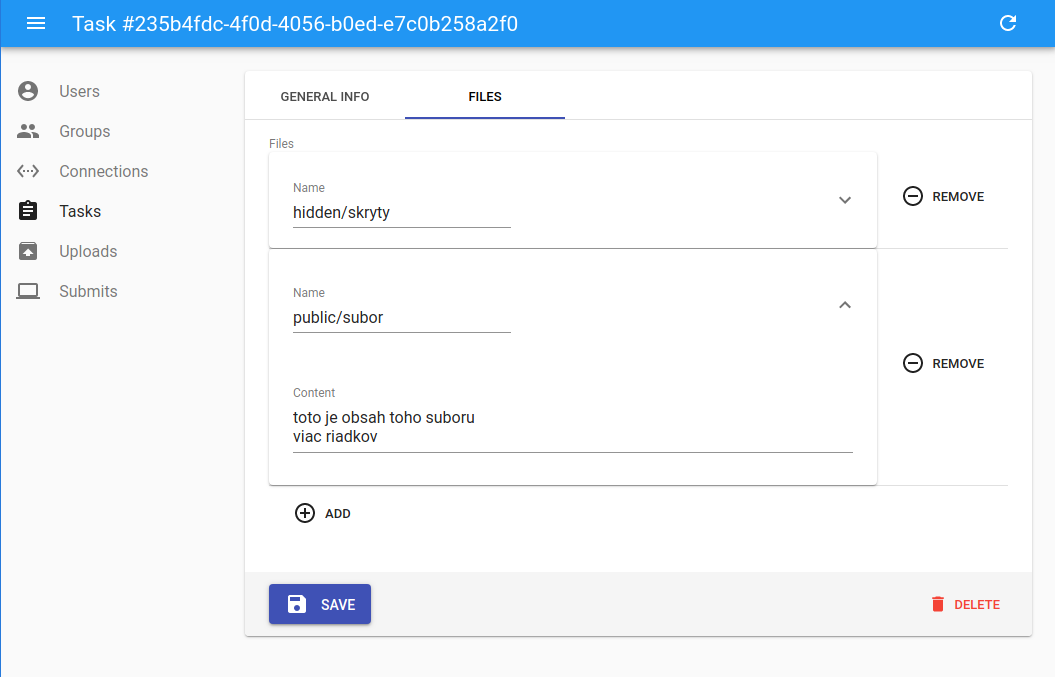
\includegraphics[width=0.8\textwidth]{images/zmena_zadania}
  \caption[Zmena zadania]{Zmena zadania}
  \label{obr:zmena_zadania}
\end{subfigure}%
\begin{subfigure}{.5\textwidth}
  \centering
  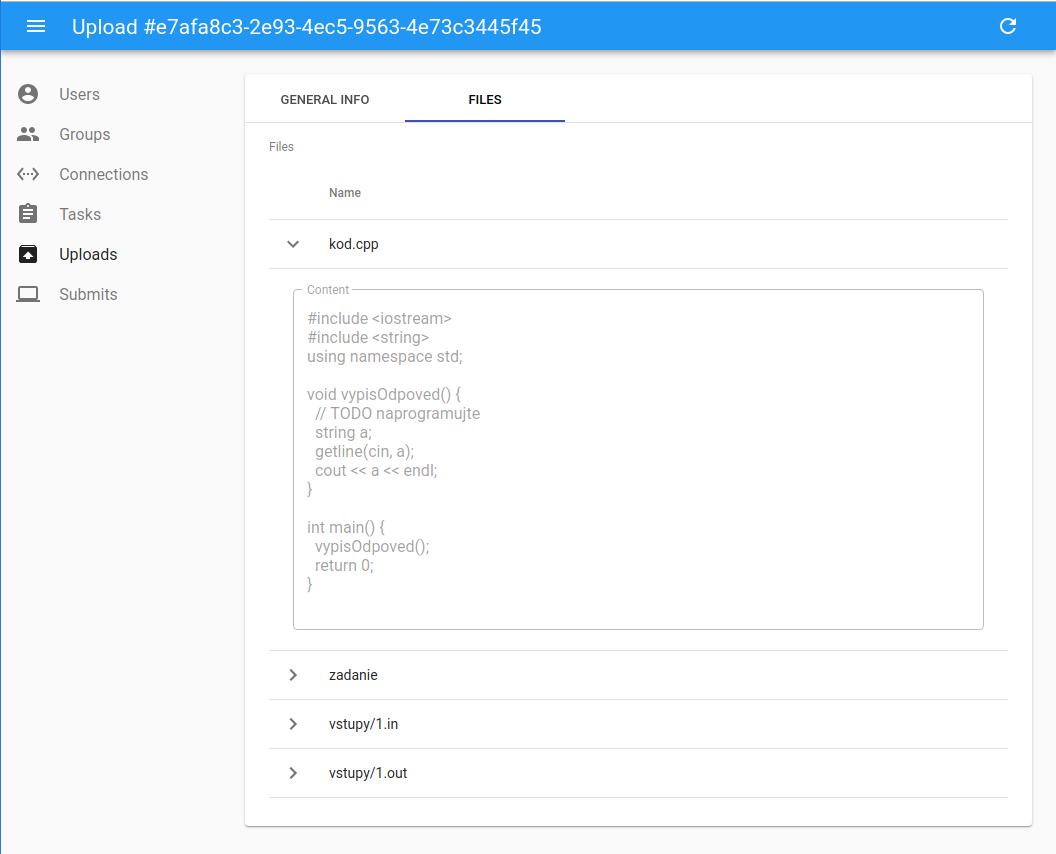
\includegraphics[width=0.7\textwidth]{images/detail_nahratia}
  \caption[Detail nahratia zadania]{Detail nahratia zadania}
  \label{obr:detail_nahratia}
\end{subfigure}
\caption{Detail entít}
\end{figure}

Tabuľka entít vie aj previazať vzťahy medzi entitami. Napríklad v prípade entity používateľov, 
zobrazené skupiny predstavú klikateľný link na detail danej skupiny. Tiež si treba uvedomiť, že
entita používateľa zo servera nedostane názov skupín ale iba identifikátory skupín. Knižnica 
však dokáže pre každý identifikátor stiahnuť dáta o skupine a potom zobraziť meno danej skupiny.
\begin{figure}[H]
\centerline{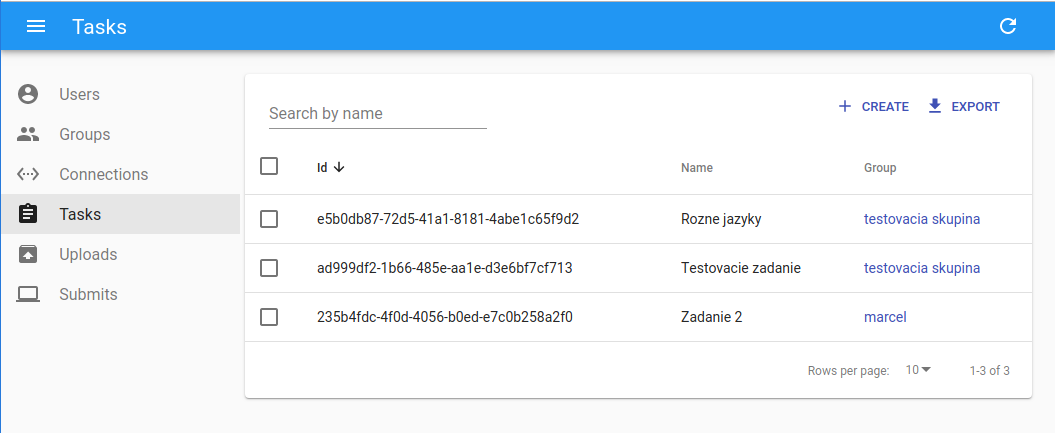
\includegraphics[width=1\textwidth]{images/zadania}}
\caption[Tabuľka zadaní]{Tabuľka zadaní}
\label{obr:zadania}
\end{figure}

% https://tex.stackexchange.com/questions/5035/paragraph-style-how-to-force-line-break-paragraph-make-paragraph-a-he
\paragraph{Stránkovanie}\leavevmode\\
V spodnej časti panela sa nachádza stránkovanie, ktoré sa využíva na to, aby v tabuľke nebolo naraz
príliš veľa výsledkov. Stránkovanie je tiež užitočné kôli šetreniu siete a rýchlosti odpovedania na
požiadavky, pretože v odpovedi na požiadavku stačí posielať menej výsledkov. Počet entít v stránke
je tiež meniteľný.

\section{Server}
Server je rovnako ako klient napísaný v jazyku Typescript. Kód napísaný v tomto jazyku sa
automaticky preloží na ekvivalentný kód jazyka JavaScript. Server potom tento kód spustí pomocou
\textit{Node.js}. Node je prostredie, ktoré slúži na spúštanie jayzka JavaScript mimo webového
prehliadača. Okrem toho Node obsahuje viaceré knižnice, ktoré nie sú dostupné v prehliadači ako
napríklad knižnica na prístup k súborovému systému alebo knižnica na spúštanie systémových volaní.
Knižnica použítá na vytvorenie webového rozhrania servera sa nazýva \textit{Express}. Express má
viaceré rozšírenia, ktoré sú dostupné ako samostatné knižnice, ktoré napríklad komprimujú odpovede
na webové požiadavky, prekladajú formát parametrov poslaných v požiadavke...

Server je zodpovedný za uchovávanie a menežovanie entít. Entity sa uchovávajú v
databáze a priamo na súborovom systéme servera. V databáze sa ukladá všetko, okrem súborov
zadania a súborov vytvorených pri ukladaní zadania. Tieto súbory sú uložené v špeciálnych
priečinkoch, ktoré majú názov rovanký ako identifikátor danej entity v databáze. To znamená, že
ak server pozná identifikátor entity, vie si jednoducho načítať aj súbory patriace k danej entite.
Použitá databáza je \textit{PostgreSQL}, pretože poskytuje viaceré pokročilé funkcie.

Webové rozhranie servera umožňuje zadávať rôzne parametre, ktoré ovpľyvňujú vrátené výsledky. Tieto
parametre slúžia ako filtre, prípadne triedia výsledky podľa nejakého stĺpca. Tieto parametre sa
posielajú databázovej vrstve, ktorá ich nastaví pri vytváraní databázovej požiadavky.

% https://tex.stackexchange.com/questions/5035/paragraph-style-how-to-force-line-break-paragraph-make-paragraph-a-he
\paragraph{Spúštací skript}\leavevmode\\
Okrem menežovania entít, je server zodpovedný aj za spúštanie kódu. Kód sa spúšta buď na vlastnom
vstupe alebo na skrytých vstupoch zadania. To ako sa má program spustiť, skompilovať a prípadne
otestovať hovorí kompilačný skript. Je to skrytý súbor, ktorý má názov
\textit{run\_script.json}. Tento súbor server načíta ešte predtým ako kód klienta spustí. Server
vďaka tomu vie tento skript pozmeniť a napríklad nastaviť aby sa kód spúštaľ na vlastnom vstupe,
ktorý rozhranie servera dostalo vo webovej požiadavke. Ak sa v kompilačnom skripte nenastaví
vlastný vstup, tak program sa postupne spustí na všetkých skrytých vstupných súboroch a porovnáva
ich výstup so správnym výstupom. Skryté súbory majú koncovku \textit{.in} a výstupné \textit{.out}.
Ak sa výstup programu nezhoduje so správnym výstupom, testovanie sa ukončí.

V spúšťacom skipte vie používateľ nastaviť viaceré parametre testovania ako napríklad spôsob
kompilácie a spúštania, časový limit...
\begin{figure}[H]
\centerline{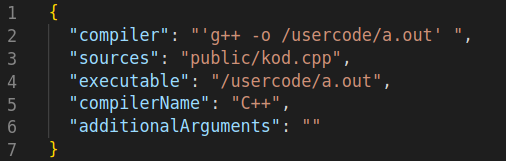
\includegraphics[width=0.8\textwidth]{images/spustaci_skript}}
\caption[Spúštací skript]{Spúštací skript}
\label{obr:zadania}
\end{figure}

\section{Izolované spúštanie kódu na serveri}
Kód spustený na serveri, nesmie narušiť ostatné bežiace programy. Klientský kód, môže obsahovať
ľubovolné príkazy jazyka, ako napríklad systémové volania, ktoré sú pre ostatné programy a stav
servera nebezpečné. Okrem bezpečnosti, je dôležité aby kódy používateľov, ktoré sa práve spúštajú
boli nezávislé.

Myšlienka testovačov pre rôzne jazyky je tu už dlho, a problematika tejto témy je hodná celej
bakalárskej práce. Rozhodli sme sa pre jednoduché riešenie, ktoré je škálovateľné pre ľubovolné
jazyky. Riešenie je založené na knižnici \textit{Compilebox}, ktorú sme mierne upravili. Základnou
myšlienkou knižnice je, že kód sa spúšta v \textit{dockeri}, ktorý zaručuje izolovanosť od ostatných
procesov na serveri. 

\subsection{Docker}
TODO:

\subsection{Spúštanie kódu}
Po nainštalovaní dockera je nutné vytvoriť dockerový obraz, ktorý obsahuje všetky podporované
jazyky. Ak na server príde požiadavka spustiť kód používateľa, vytvorí sa súbor do ktorého sa
nakopírujú všetky súbory potrebné na testovanie. Klient má ale iba prístup k verejným súborom ale
pri testovaní potrebujeme aj skryté súbory zadania. Pri spúštaní programu ale vieme, ktoré zadanie
používateľ rieši a teda vieme, ktoré skryté súbory skopírovať. Názov súboru je unikátky
identifikátor, ktorý zaručuje nezávislosť spúštania viacerých programov naraz. Keď sú všetky súbory
pripravené, z dockerového obrazu sa vytvorí kontajner, v ktorom sa kód skompiluje a spustí. Výstup
programu z testovania je presmerovaný do výstupného súboru a prípadné chyby alebo varovania pri
kompilácii, či behu programu sa zapisujú do samostatných súborov, ktoré kontajner vytvorí. Po
dokončení behu programu kontajner vytvorí špeciálny súbor, ktorý označuje ukončenie behu programu.
Server pravidelne kontroluje, či daný súbor existuje. Server úmyslne nečaká kým sa spustený program
v dockeri neskončí, pretože nič nezaručuje, že klientský program niekedy skončí. Vďaka takémuto
riešeniu vieme implementovať aj časový limit programu, kde po prekročení daného limitu bežiaci
program ukončíme. Po skončení behu programu vrátime obsah súborov serveru, a celý priečinok, v
ktorom boli potrebné súbory na spúštanie vymažeme.
